\documentclass[10pt]{beamer}
\usetheme[
%%% options passed to the outer theme
%    progressstyle=movCircCnt,   %either fixedCircCnt, movCircCnt, or corner
%    rotationcw,          % change the rotation direction from counter-clockwise to clockwise
%    shownavsym          % show the navigation symbols
  ]{AAUsimple}
% If you want to change the colors of the various elements in the theme, edit and uncomment the following lines
% Change the bar and sidebar colors:
%\setbeamercolor{AAUsimple}{fg=red!20,bg=red}
%\setbeamercolor{sidebar}{bg=red!20}
% Change the color of the structural elements:
%\setbeamercolor{structure}{fg=red}
% Change the frame title text color:
%\setbeamercolor{frametitle}{fg=blue}
% Change the normal text color background:
%\setbeamercolor{normal text}{fg=black,bg=gray!10}
% ... and you can of course change a lot more - see the beamer user manual.

\usepackage[utf8]{inputenc}
\usepackage[english]{babel}
\usepackage[T1]{fontenc}
% Or whatever. Note that the encoding and the font should match. If T1
% does not look nice, try deleting the line with the fontenc.
\usepackage{helvet}
\usepackage{graphicx} %For figures
\graphicspath{{./images/}}
\usepackage{tikz} %Tikz
\usepackage{tikzscale}
\usepackage{tikz-uml}
\usetikzlibrary{calc, arrows, decorations.markings,decorations.text, shapes, positioning}
\usepackage{pgfplots} %Graph plotting
\pgfplotsset{compat=newest,
  table/col sep = comma,
  every axis legend/.append style={
    no marks,
    filter discard warning=false,
  }
}
\usepackage{siunitx}

% colored hyperlinks
\newcommand{\chref}[2]{%
  \href{#1}{{\usebeamercolor[bg]{AAUsimple}#2}}%
}
\newcommand{\perc}[1]{\SI{#1}{\percent}}

\title{Point and Control with Gestures in a Smart Home}

% \subtitle{v.\ 1.3.2}  % could also be a conference name

\date{\today}

\author{
  Jens Emil Gydesen\\ \href{mailto:jgydes11@student.aau.dk}{{\tt jgydes11@student.aau.dk}}\\
  Kasper Lind Sørensen\\ \href{mailto:klsa11@student.aau.dk}{{\tt klsa11@student.aau.dk}}\\
  Simon B. Støvring\\ \href{mailto:sstavr11@student.aau.dk}{{\tt sstavr11@student.aau.dk}}
}

% - Give the names in the same order as they appear in the paper.
% - Use the \inst{?} command only if the authors have different
%   affiliation. See the beamer manual for an example

\institute[
%  {\includegraphics[scale=0.2]{aau_segl}}\\ %insert a company, department or university logo
  Dept.\ of Computer Science\\
  Aalborg University\\
  Denmark
] % optional - is placed in the bottom of the sidebar on every slide
{% is placed on the bottom of the title page
  Department of Computer Science\\
  Aalborg University\\
  Denmark
  
  %there must be an empty line above this line - otherwise some unwanted space is added between the university and the country (I do not know why;( )
}

% specify a logo on the titlepage (you can specify additional logos an include them in 
% institute command below
\pgfdeclareimage[height=1.5cm]{titlepagelogo}{AAUgraphics/aau_logo_new} % placed on the title page
%\pgfdeclareimage[height=1.5cm]{titlepagelogo2}{AAUgraphics/aau_logo_new} % placed on the title page
\titlegraphic{% is placed on the bottom of the title page
  \pgfuseimage{titlepagelogo}
%  \hspace{1cm}\pgfuseimage{titlepagelogo2}
}

\begin{document}
% the titlepage
{\aauwavesbg%
\begin{frame}[plain,noframenumbering] % the plain option removes the header from the title page
  \titlepage
\end{frame}}
%%%%%%%%%%%%%%%%

% TOC
\begin{frame}{Agenda}{}
\tableofcontents
\end{frame}
%%%%%%%%%%%%%%%%

\chapter{Introduction}\label{chap:introduction}
In recent years there has been a large increase in so-called \emph{smart devices}. 
A smart device is an electronic device that is connected to one or more other smart devices. 
Common protocols for the interconnection of smart devices are WiFi or Bluetooth, among others.
Smart devices are part of a concept called the Internet of Things, or IoT. 
IoT is a concept describing a network of physical devices, such as smart devices. 
Example of devices that are part of a network could be a coffee machine, a watch or even a refrigerator. 
Devices such as smartphones, laptops or servers, that are already commonly connected to the Internet, are usually not considered part of this IoT network. 

The IoT network recently became a reality when the IPv6 protocol was launched,
creating a total of $2^{128}$ unique IP addresses, 
so that devices such as a smart coffee machine could get its own unique IP address. 
One of the companies that quickly accepted IoT is Coca-Cola, 
who, already by 2010, reserved $16$ million IP addresses to use for \eg their vending machines around the world \cite{coke-iot}. 

We will use the remainder of this chapter to explore the technologies and uses of IoT. 
We start by analyzing wearables, \ie smart devices that are worn, in \Cref{sec:wearables}.
Another large part of IoT is the concept of smart homes, \ie homes that are partially or fully automated by utilizing smart technologies and devices. 
We will analyze this in \Cref{sec:smarthomes} where \Cref{sec:system-categories} describes different levels of home automation. 
Indoor location, described in \Cref{sec:indoor-positioning}, can play an important part in smart homes and automation.
Finally we propose a problem statement \Cref{sec:researchstatement} and give an overview of the rest of the report in \Cref{sec:overview}.

\section{Wearables}\label{sec:wearables} %Working title
%Thalley: Første source kan også laves som en fin graf hvis ønsket. Brug tal fra: http://www.statista.com/statistics/259372/wearable-device-market-value/
Wearable technology is a trending form of technology as of 2015 \cite{WEARABLESTREND}. 
As the name implies, wearables are devices that, unlike most electronics, are worn by the user. 
The most common types of wearables today are smartwatches, 
\ie watches that run an advanced operating system and can perform more actions that regular watches such as communicating with a smartphone or other smart devices, 
and smart wristbands which usually tracks activity, 
among other things, and sends this data to a connected smartphone via an application. 
Smartphones are usually not considered a wearable since they are usually \emph{carried} and not \emph{worn}. 

%Hvorfor wearables?
The increasing trend in wearables is likely due to increased computational power in small devices and decreased sizes of sensors, 
which allows more power and functionality to wearables devices. 
The increasing trend, as well as better wearables devices, 
opens up new possibilities since we can now carry more computational power with us on the go that we can utilize to perform actions that we could not before, 
or perform other actions faster or better. 
Examples of this could be that we can now track our level of activity together with our location to analyze ourselves or even automate actions based on our location, mood or even health. 

%HVad kan en wearable? Hvilke sensorer findes der? Hvad er state of the art? 
If we take a look at some of the current state of the art or the most popular wearable devices right now, 
we can create an image of what we can actually monitor, track, control or in other ways do with devices that we can wear. 
One of the latest and most advanced wearable is the HIRIS \cite{hirisweb}. 
The HIRIS is a wearable computer able to track 3D movements in real-time. 
By using several HIRIS, you can get a create a full-body tracking system. 
Aside from 3D tracking, HIRIS also tracks heart rate and temperature and can connect to other devices and control these. 
Another advanced wearable tracker is the Jawbone UP3 \cite{JAWBONE}. 
This wearable is also able to track your heart rate, activity, sleep and temperature, but unlike the Hiris cannot control any other devices. 
Since one of the most popular wearables is the smartwatch, it makes sense to mention these as well. 
One of most interesting smartwatches, due to developer options, is the Pebble Smartwatch \cite{PEBBLE}. 
This smartwatch works with iPhones and Android smartphones and comes with a variety of applications for tracking fitness and control music among other things. 
Aside from this, the watch also comes with an accelerometer and a magnetometer, meaning that is can track your motions and directions. 

By analyzing the list of 348 different wearables from Vandrico\cite{LISTOFWEARABLES} of September 2015, 
we can see which sensors and components are most common among wearables and where on the body they are worn. 
It is important to note that all of this information comes Vandrico's database, and may differ from other findings. 
\Cref{fig:wearables-category} shows which categories these wearables fit in. The most common one, lifestyle, 
describes wearables such as smartwatches or other devices that are meant to be used and worn on a daily basis. 
Some devices may fit more than one category.

\begin{figure}[!htb]
    \centering
    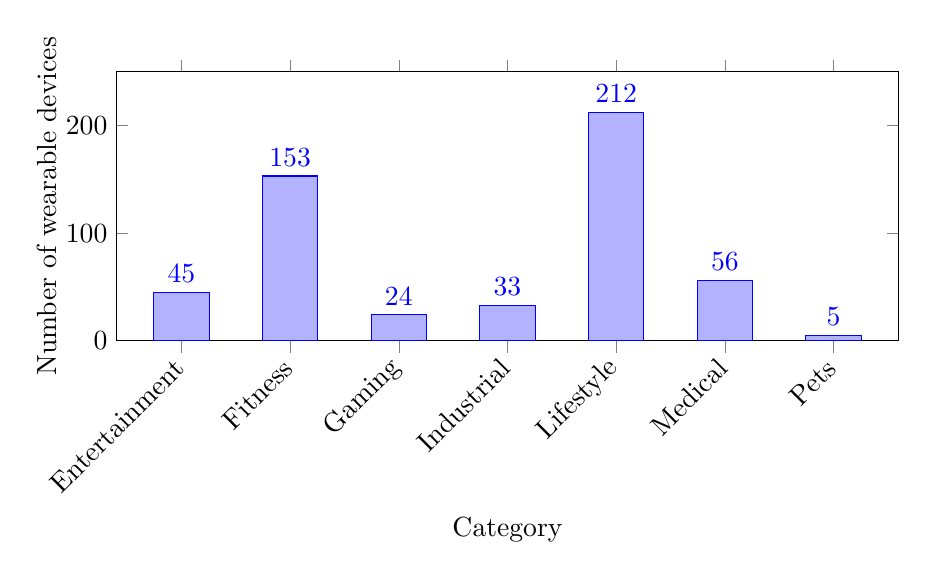
\begin{tikzpicture}
    \begin{axis}[
        height=5cm,
        width=0.95\textwidth,
        xlabel={Category},
        xticklabel style={rotate=45, anchor=east, yshift=-0.5ex},
        ylabel={Number of wearable devices},
        yticklabel style={align=right,inner sep=0pt,xshift=-0.3em},
        nodes near coords align={vertical},
        nodes near coords,
        xtick=data,
        symbolic x coords={Entertainment,Fitness,Gaming,Industrial,Lifestyle,Medical,Pets},
        ybar,
        ymax=250,
        ymin=0,
        bar width=20pt,
        ]
        \addplot coordinates {(Entertainment,45) (Fitness,153) (Gaming,24) (Industrial,33) (Lifestyle,212) (Medical,56) (Pets,5)};
    \end{axis}
\end{tikzpicture}
    \caption{Number of devices in each category}
    \label{fig:wearables-category}
\end{figure}

\Cref{fig:wearables-placement} shows where on the body the wearable should or can be worn. 
The most common placement is the wrist where smartwatches or wristband are worn, 
which are the most popular wearables. The devices that are worn on the head are usually augmented/virtual reality headsets, 
but also includes smart bike-helmets or ear/headphones.

\begin{figure}[!htb]
  \centering
  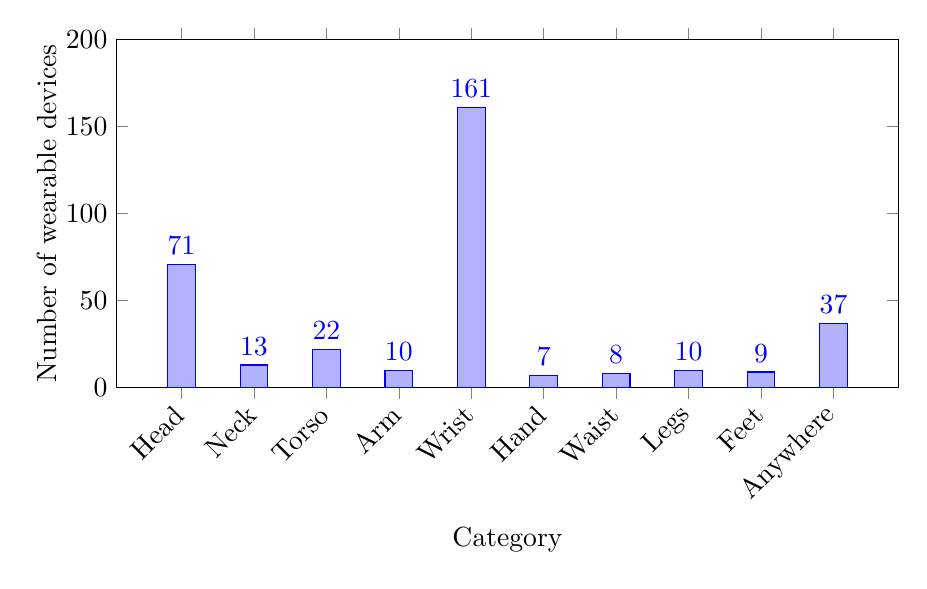
\begin{tikzpicture}
\begin{axis}[
    height=6cm,
    width=0.95\textwidth,
    xlabel={Category},
    xticklabel style={rotate=45, anchor=east, yshift=-0.5ex},
    ylabel={Number of wearable devices},
    yticklabel style={align=right,inner sep=0pt,xshift=-0.3em},
    nodes near coords align={vertical},
    nodes near coords,
    xtick=data,
    symbolic x coords={Head,Neck,Torso,Arm,Wrist,Hand,Waist,Legs,Feet,Anywhere},
    ybar,
    ymax=200,
    ymin=0,
    ]
    \addplot coordinates {(Head,71) (Neck,13) (Torso,22) (Arm,10) (Wrist,161) (Hand,7) (Waist,8) (Legs,10) (Feet,9) (Anywhere,37)};
\end{axis}
  

\end{tikzpicture}
  \caption{Placements of wearables}
  \label{fig:wearables-placement}
\end{figure}

\Cref{fig:wearables-sensors} shows which sensors and components are mostly available in wearables. 
Due to its high usability, the accelerometer is a very important sensor which is found in approximately half the wearables. 
The remaining sensors in \Cref{fig:wearables-sensors} are, unsurprisingly sensors that we also find in smartphones as they give a lot of options when it comes to developing applications. 
\begin{figure}[!htb]
    \centering
    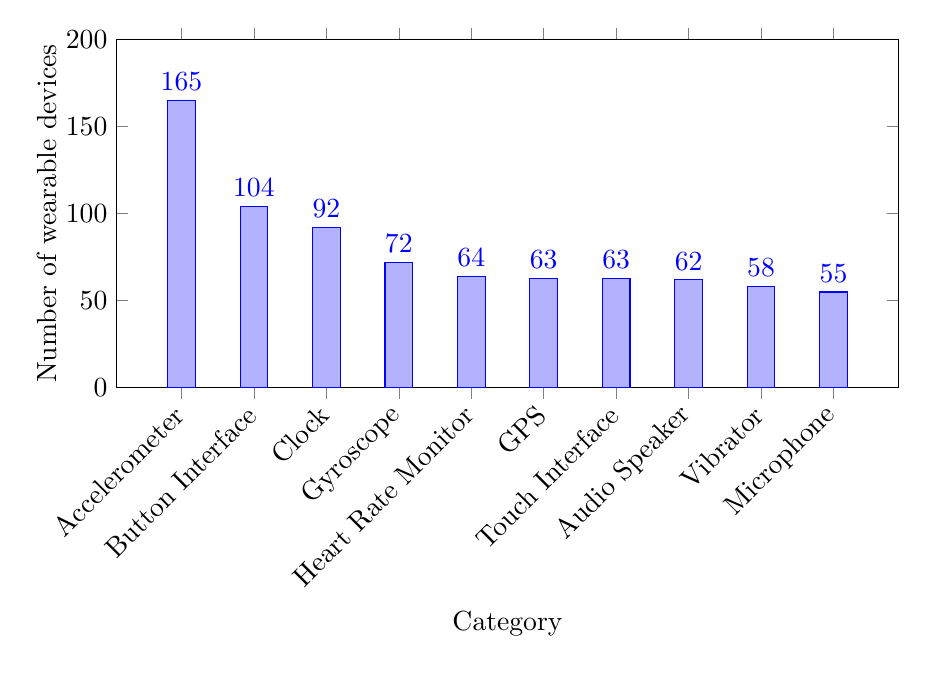
\begin{tikzpicture}
\begin{axis}[
    height=6cm,
    width=0.95\textwidth,
    xlabel={Category},
    xticklabel style={rotate=45, anchor=east, yshift=-0.5ex},
    ylabel={Number of wearable devices},
    yticklabel style={align=right,inner sep=0pt,xshift=-0.3em},
    nodes near coords align={vertical},
    nodes near coords,
    xtick=data,
    symbolic x coords={Accelerometer,Button Interface,Clock,Gyroscope,Heart Rate Monitor,GPS,Touch Interface,Audio Speaker,Vibrator,Microphone},
    ybar,
    ymax=200,
    ymin=0,
    ]
    \addplot coordinates {(Accelerometer,165) (Button Interface,104) (Clock,92) (Gyroscope,72) (Heart Rate Monitor,64) (GPS,63) (Touch Interface,63) (Audio Speaker,62) (Vibrator,58) (Microphone,55)};
\end{axis}
  

\end{tikzpicture}
    \caption{Top 10 mostly used sensors}
    \label{fig:wearables-sensors}
\end{figure}

This section gave a short overview of the current state of wearables, what they are and which sensors are widely available. 
This information should be remembered if developing any system that utilizes wearables. 

%Skab et overblik over de nyeste devices
%Grafer over hvilke sensorere der mest typiske?
%Grafer over kropsdele?
%Hvad er de nyeste teknologier indenfor wearables? 

\section{Smart Homes}
Another trend that utilizes the concept of IoT is smart homes which are homes that are, to some degree, automated by utilization IoT devices. 
The devices used for smart homes differ greatly from wearables as they are usually stationary. 
The concept of smart homes have been around for a while and numerous homes have already integrated some of these smart devices. 
A good example of a high-end smart home is Bill Gate's mansion in Medina, Washington \cite{billgatehouse}.
This \$100 million house have sensors to adjust each room's temperature and lighting and have speakers behind the wallpaper that follows you from room to room. 
The artwork in the house is mostly digital and can be changed by pressing a button. 
One can only imagine what other technology is being used in that house. 

However, that is a rather extreme example of a smart home. 
Ordinarily, the devices found in smart homes are common items that has been connected to the Internet for wireless control.
Common devices that are found in smart homes include, but are not limited to, 
coffee machines, washers and dryers, thermostats, sound systems and locks. 
However, only few devices have really gained ground for the common user and few homes are automated.
One of the most commonly found IoT in homes are the Nest thermostat \cite{NEST}. 
This thermostat senses when you are around and when you are not to control the climate inside to save energy and thus money.
Unlike a lot of smart devices that are made to make your life a little easier, such as an automated coffee machine, 
the Nest thermostat helps you save money which is likely the reason for it popularity. 
Furthermore, the newest version (as of October 2015) allows you to connect other IoT devices to the thermostat. 
The Nest thermostat is thus starting to solve what is probable the greatest problem with smart homes (and IoT in general) and why they have not become popular yet: Lack of interconnectivity between IoT devices. 

\subsection{Smart Hubs}
%Something about SmartThings
%How does wearables fit in

\subsection{Indoor Positioning}\label{sec:indoor-positioning}
%Something about Estimote
In order to determine which device the user points at and thereby intends to control, 
it is necessary to determine the locations of the devices in the system relative to the user.

The focus of this project is not to position devices and as such it was not the intention to spend time developing an entire solution for positioning devices indoors. 
Instead it was desired to find an existing product that could be used to facilitate indoor positioning.
The solution should be available in the early phases of the project in order to start building the system based on the solution for positioning.

Ideally users of this project should be able to control any device that fits within the concept of Internet of Things he owns, 
the price for any device needed to position each controllable device should be low. 
If a user owns several devices that can be controlled using gestures and an extra device is needed for each in order to preform the positioning, 
the price of such a device should be at a minimum.

It is assumed that users already own one or more devices that fit within the concept of Internet of Things and possibly are early adapters of such technology, 
it is assumed they have some technological expertise. 
However, it easy to imagine that this project can be used in an office environment where employees of varying technological expertise work or in health care. 
Therefore users may have a varying degree of technological expertise and it should be easy to extend the solution with new controllable devices.

Naturally the accuracy of the solution used for positioning objects plays an important part. 
\Cref{fig:indoor-positioning:incorrect} shows the consequence of an incorrect location. 
If a lamp is estimated to be at another location that it is actually located, 
the user must point to an incorrect location in order to control the lamp.
Furthermore if the estimate is too wide, that is, the given area in which the lamp is located is very big, 
there is a greater risk that locations overlap. 
Overlapping locations causes a complexity as it is necessary to determine which device the user desires to control if he points at the overlap as visualized in figure \ref{fig:indoor-positioning:overlap}.

\begin{figure}[h]
    \centering
    \includegraphics[height=5cm]{images/incorrect-positioning-estimate.png}
    \caption{Incorrect location estimate. The estimate is visualized as a striped circle.}
    \label{fig:indoor-positioning:incorrect}
\end{figure}

\begin{figure}[h]
    \centering
    \includegraphics[height=5cm]{images/positioning-overlap.png}
    \caption{Overlap of estimated positions. The estimates are visualized as a striped circle.}
    \label{fig:indoor-positioning:overlap}
\end{figure}

Based on the above the following criteria for assessing potential solutions can be outlined.

\begin{itemize}
    \item Availability
    \item Price
    \item Ease of use
    \item Accuracy
\end{itemize}

Only solutions intended for indoor positioning was considered and thus GPS is not considered a potential solution. 
GPS is meant for outdoor positioning and a signal is not always available while indoors and even if it is, the accuracy of the estimated location is very low.

\begin{table}[h]
    \centering
    \caption{Assessment of potential solutions for indoor positioning. Please not that all prices are converted to U.S. dollars from their respective currency. Prices include the minimum available hardware for positioning a device.}
    \label{tbl:indoor-positioning}
    
    \begin{tabularx}{\textwidth}{XXXXX}
        \textbf{Product} & \textbf{Availability} & \textbf{Price} & \textbf{Ease of use} & \textbf{Accuracy} \\
        
        Estimote Beacons and Stickers \cite{estimote}
        & Beacons and Stickers are shipping. SDKs available.
        & \$99 for beacons. \$99 for 10 stickers, one per device to be positioned.
        & Initial installation of beacons. Attach each sticker to device.
        & Unknown. Desired to be less than five meters. \todo[author=Simon]{Update after conducting tests.} \\
        
        Pozyx \cite{pozyx}
        & Available for preorder.
        & \$368 for anchors. \$123 for each device to be positioned, plus supported Arduino.
        & Initial installation of anchors. One tag for each device, plus supported Arduino. Not meant for mounting.
        & Claimed to be 10 cm. Untested.
        
    \end{tabularx}
\end{table}

%%% Local Variables:
%%% mode: latex
%%% TeX-master: "../../master"
%%% End:

\section{System Categories}\label{sec:system-categories}
Smart home automation is one of the big sell-points of smart homes.
Home automation can happen at various degrees. 
In this section we will analyze and categorize the different types of smart home automation. 

The scenarios in which home automation is facilitated can in general be divided into the following three categories.

\begin{enumerate}
    \item Rule driven systems
    \item Gesture driven systems
    \item Autonomous systems
\end{enumerate}

The categories varies in the way users configure and interact with the systems. 
``Manual systems'' could constitute a fourth category, consisting of regular systems with manual switches,
but is left out as it such systems do not contribute to home automation.
Each of the three categories and their use cases are briefly described below.

\subsection{Rule Driven Systems}

A system is considered to be rule driven if an action is executed when a set of rules are fulfilled. 
The rule driven systems use conditional statements to express input and output. 
Below are a few examples of rules in the form of (if this) \textrightarrow (then that):

\begin{itemize}
    \item (The temperature is above 23 degrees Celsius) \textrightarrow~(Lower the temperature on my thermostat)
    \item (The CO\textsubscript{2} index is critically high) \textrightarrow (Open my windows)
\end{itemize}

The above rules consist of a condition on the left-hand side of the arrow and an action on the right-hand side of the arrow.
The automation of the smart home is based on the set of rules. 
To achieve the desired behavior, the user must add, remove or tweak existing rules.

Examples of rule drive systems include the aforementioned Apple HomeKit. 
As outlined in the framework reference for HomeKit \cite{applehomekitref}, the system is based on actions and events. 
Triggers constitutes rules by encapsulating actions and events. 
Each event represents a condition. 
An event may be fulfilled by a change in time, the state of devices in the system of the location of the user.

\subsection{Gesture Driven Systems}

Systems are gesture driven if the system is configured with a set of gestures that can be performed by the user in oder to trigger some action. 
Each device in the system responds to a set of gestures. 
For example, a lamp may respond to the user waving in order to turn on and the user clapping in order to turn off.

A gesture driven system is partly rule driven as each gesture registered in the system is associated with one or more actions. 
The association means that each time the gesture is registered in the system, the action should be triggered. 
Such rules can be formulated as ``if I wave, then lower the temperature on my thermostat''

Examples of gesture driven systems includes Hiris, a wearable computer with focus on gestures that allow the users to interact with other devices \cite{hirisweb}.

\subsection{Autonomous Systems}

An autonomous system monitors the system and proactively responds to changes in the system. 
Observable changes include but are not limited to changes in the temperature, CO\textsubscript{2} index, the number of people in the room or even who are in the room.
Autonomous systems should intelligently react to the users needs based upon the observable state of the environment.

Autonomous systems rely on the concept of ambient intelligence in order to determine the necessary actions.
\todo[author=Thalley]{Maybe add something about ambient intelligence here?}
Such systems include autonomous enhancement services that replaces manual care with an automated system \cite{nehmer2006living}. 
These systems gather environment and the data about the individuals body functions, 
\eg temperature, pulse and blood pressure in order to determine if the individuals health is critical.

Autonomous systems are rule driven systems that intelligently determines the rules to be created and the necessary action to take when a set of rules are fulfilled. 
Typical for such systems may be the complexity of the rules. 
It is not given that users themselves are capable of determining a suitable set of rules in order to judge if their health is critical. 
The system should itself be able to determine such set of rules and adjust it to the individual.

Examples of autonomous systems include the one described Nehmer \etal\cite{nehmer2006living}. 
The authors envision a living assistance system which monitors elderly people. 
A model is outlined and by continuously feeding the model with data about the individuals body functions and his behavior, 
they can determine if a \emph{critical situation} occurs. 
A critical situation could be that the person has fallen and are not responding to contact, for example calls.
Such system may reduce the cost of providing care to the elderly people.

\subsection{Conclusion}

The rule driven, gesture driven and autonomous systems are all rule driven to some extend but the origin and the types of rules differ between the systems. 
In a rule driven system the rules are configured by the user.
In an autonomous system the rules are programmed by some expert or in collaboration with experts in a certain field, \eg the medical field. 
The system may adapt its set of rules based on the environment and that behavior of the individual.
Gesture driven systems use rules configured by the user. 
In such systems gestures make up the condition of a rule.

When concerned with the field of home automation it is relevant to classify each system in order to determine how automatic a system is. 
The more automatic a system is, the less the user should be involved with the system.

The degree of automation as well as the reasoning behind each of the classifications are shown in \Cref{tbl:system-categories}.

\begin{table}[h]
    \centering
    \begin{tabularx}{\textwidth}{XXX}
    \textbf{Gesture driven systems}       & \textbf{Rule driven systems}                             & \textbf{Autonomous systems} \\
    \textit{Lowest degree of automation}  & \textit{Medium degree of automation}                     & \textit{Highest degree of automation}\\
    Configured by the user.               & Configured by the user.                                  & Configured by an expert.\\
    Conditions are triggered by the user. & Automatically and constantly observes the environment.   & Automatically and constantly observes the environment.\\
    ~                                     & The configuration may be reusable for other individuals. & Automatically adjusts to the users needs.\\
    \end{tabularx}
    \caption{Classification of systems based on their degree of automation}
    \label{tbl:system-categories}
\end{table}

%%% Local Variables:
%%% mode: latex
%%% TeX-master: "../../master"
%%% End:

\section{Indoor Positioning}\label{sec:indoor-positioning}
One of the most discussed or wanted features in an automated smart home, 
is having the smart home detect where you are.
There are multiple use cases for this feature, 
not only in smart homes, but also in a lot of other settings. 
A few examples of where indoor positioning, or location, can be useful:
\begin{enumerate}
    \item Indoor navigation (\eg in large publics buildings such as airports or hospitals)
    \item Tracking of patients in \eg hospitals or elderly care facilities
    \item Finding lost objects such as keys in a home
    \item Tracking people in smart homes to execute certain actions when a person is near an object or an area
\end{enumerate}

%Something about Estimote

\section{Problem Statement}
In the previous sections we analyzed different areas of Internet of Things (IoT) including how wearables and home automation are maturing. 
We have seen some of the possibilities of wearables and we can see that this can integrated with home automation and indoor location.
We think that exploring the concept of home automation with wearables can result in a usable system that better utilizes the devices for smart homes by giving a better interface. 
More accurately, we want to explore the possibilities of interconnecting smart devices using existing technologies.
In the remainder of this report, we will answer the following question:
\begin{framed}
    \begin{quote}
        What can we do with wearables and smart devices in a smart home setting, where different smart devices may use different communication protocols?
        
        In answering this question, we will also answer the following questions:
        \begin{itemize}
            \item What problems arise when working with different platforms using different operating systems?
            \item Which limitations does current technology have in the area of IoT? Can we overcome it and how? 
           \end{itemize} 
    \end{quote}
\end{framed}
%Thalley: For meget med frame? Evt. bruge noget andet for at fremhæve problemformuleringen, eller bare droppe det helt? 


%Thalley: Gammel formulering:
%\begin{quote}
%    \begin{itemize}
%        \item Explore the possibilities of interconnecting smart devices using existing technologies  
%        \item Give users a better interface of controlling smart devices with gestures using a wearable in a smart home 
%    \end{itemize}    
%\end{quote}
%
%The goal of our research is to create a system that allows gesture-based communication between the user and smart devices.
%We feel that allowing users to point and control devices will give the best interface. 
%This approach requires accurate indoor location, a wearable that can recognize gestures and a hub for interoperability between the wearable and the smart devices. 
\section{Overview}\label{sec:overview}
This section will briefly describe the structure and the content of rest of the report. 
This report consists of 6 chapters and should be read from Chapter 1 through Chapter 6. 
The first chapter, \Cref{chap:introduction}, which you have just read, 
was an introduction to the problem domain, 
briefly exploring existing technologies in the area of IoT. 
In \Cref{chap:analysis} we further analyze the problem, 
and existing solutions.
\Cref{chap:design} describes the architecture and design of our system. 
The system's implementation, and prototypes during the project, 
will be described in \Cref{chap:implementation}.
Then we evaluate our system in \Cref{chap:evaluation}, 
to see if it meets the requirements from \Cref{sec:requirements-specification}.
Lastly, we end this report by making a conclusion in \Cref{chap:conclusion}, 
where we show and discuss the final results, 
and discuss how the system may be further improved. 


\section{Architecture}

% Architecture
\begin{frame}{Architecture}{}
\centering
\begin{figure}
  \scalebox{0.75}{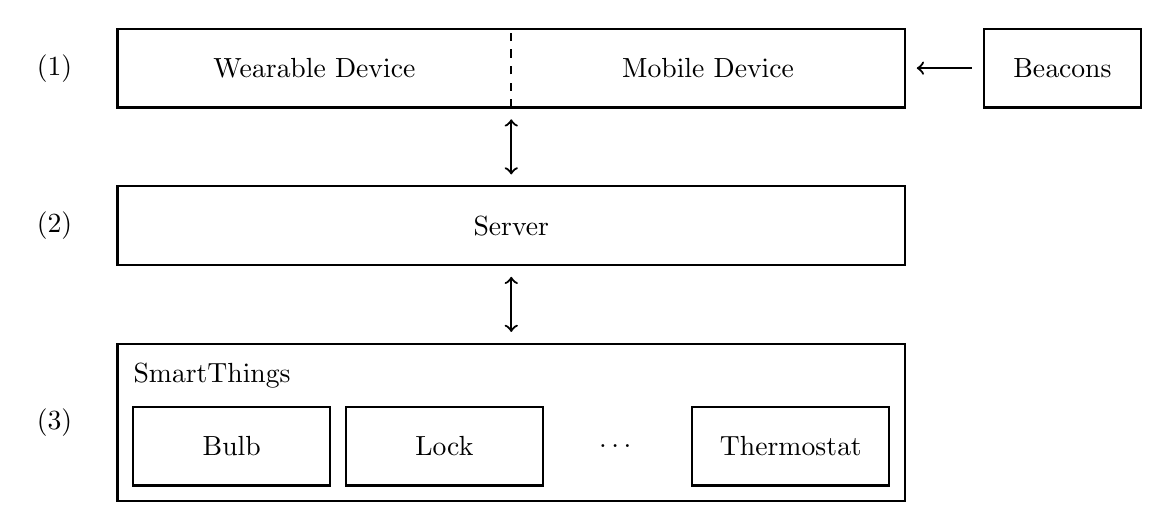
\begin{tikzpicture}
    \node[anchor=center] at (-0.8,0.5) {(1)};
    \node[anchor=center] at (-0.8,-1.5) {(2)};
    \node[anchor=center] at (-0.8,-4) {(3)};
    
    \node[anchor=center] at (2.5,0.5) {Wearable Device};
    \node[anchor=center] at (7.5,0.5) {Mobile Device};
    \draw[thick] (0,0) rectangle (10,1);
    \draw[thick, dashed] (5,0) -- (5,1);
    \draw[thick,->] (10.85,0.5) -- (10.15,0.5);
    \draw[thick] (11,0) rectangle (13,1) node[pos=.5] {Beacons};
    
    \draw[thick] (0,-1) rectangle (10,-2) node[pos=.5] {Server};
    \draw[thick,<->] (5,-0.15) -- (5,-0.85);
    
    \node[anchor=center] at (1.2,-3.4) {SmartThings};
    \draw[thick] (0,-3) rectangle (10,-5);
    \draw[thick,<->] (5,-2.15) -- (5,-2.85);
    \draw[thick] (0.2,-3.8) rectangle (2.7,-4.8) node[pos=.5] (bulb) {Bulb};
    \draw[thick] (2.9,-3.8) rectangle (5.4,-4.8) node[pos=.5] (lock) {Lock};
    \draw[thick] (7.3,-3.8) rectangle (9.8,-4.8) node[pos=.5] (door) {Thermostat};
    \node at ($(lock)!.5!(door)$) {\ldots};
\end{tikzpicture}}
\end{figure}
\end{frame}

% HomePort
% \begin{frame}{Architecture}{HomePort}
% \centering
% \begin{figure}
%   \subfloat{
%     \includegraphics[width=0.48\textwidth]{../images/phidget_off}
%   }
%   \subfloat{
%     \includegraphics[width=0.48\textwidth]{../images/phidget_on}
%   }
% \end{figure}
% \end{frame}

%%% Local Variables:
%%% mode: latex
%%% TeX-master: "../AAUsimpletheme"
%%% End:

\chapter{Evaluation}\label{chap:evaluation}
\todo[author=Thalley]{Write about test setup. Which devices we use and their specs}
\section{Performance of Gesture Recognition}\label{sec:gestureperformance}
Gesture recognition is a core part of our solution and it is being performed often. 
Since the gesture recognition is being performed by a device with somewhat low performance,
it is important that the gesture recognition is not computationally heavy.
In \Cref{sec:requirements-specification} we set a requirement of less than \SI{200}{\milli\second} for each gesture recognition.
We test the performance by gradually populating the database with gesture traces, 
and see how fast we can recognize a random gesture input.
We expect the number of gesture traces in the database to increase the recognition time.

For this setup, we add five gesture traces at a time. 
This is to simulate training a gesture five times, 
as recommended by the \$3 Gesture Recognition paper \cite{threedollar}. 
We then generate a random gesture input, 
and run the recognition function on it ten times, 
logging the execution time.
We repeat this until there is a total of \num{100} gesture traces in the database, 
which corresponds to \num{20} unique gestures.

We performed this test six times on an iPhone 5, 
with a \SI{1.3}{\giga\hertz} dual-core ARM processor and \SI{1}{\giga\byte} RAM, running iOS 9.1.
This device is more powerful than most wearables, 
but newer wearables such as the Samsung Gear S2 has a \SI{1}{\giga\hertz} dual core CPU with \SI{512}{\mega\byte} RAM, 
so the results from this section are comparable with newer and upcoming wearable devices.

\begin{figure}[!htb]
    \centering
    \begin{tikzpicture}
  \begin{axis}[ybar,bar width=2pt]
    \addplot table[x=gestureNo, y=time] {data/three-dollar-test-results/results/10xrecognize/2015-11-25 12.36.29.csv};   
  \end{axis}
\end{tikzpicture}
    \caption{Graph showing the time of recognizing gestures, with increasing number of gesture traces. Each unique gesture is training \num{5} times.}
    \label{fig:performancegraph}
\end{figure}

During testing we noticed that the ``Three Dollar Gesture Recognizer'' used a high amount of memory. 
Furthermore it did not properly release this memory, 
and as a result the application would terminate during tests, 
if we ran them for too long.
\Cref{fig:threedollarmemory} shows the amount of memory, 
used by our application, 
in a timespan of one minute and thirteen seconds, 
starting at the point where the application was launched on the iPhone. 
The first dotted line shows the time when the test began, 
and the second dotted line shows when the test finished, 
and where the \$3 Gesture Recognizer started cleaning up its resources.
However, as the graph shows, the memory use stays high after cleanup. %Thalley: Kunne det ikke blot være pga. iOS's måde at håndtere memory på? 
This issue is the reason we only repeat recognition ten times for each gesture, 
as more would cause the application to shut down due to excessive memory usage. %Thalley: Kan vi se hvor mange gestures den højst kan recognize før det er et problem? 

\begin{figure}[!htb]
  \begin{tikzpicture}
    \centering
    \node[anchor=south west,inner sep=0] (image) at (0,0) {\includegraphics[width=0.7\textwidth]{images/three-dollar-memory-use.png}};
    \begin{scope}[x={(image.south east)},y={(image.north west)}]
    \draw[red,ultra thick, dotted] (0.45,0.08) -- (0.45,0.97);
    \draw[red,ultra thick, dotted] (0.73,0.08) -- (0.73,0.97);
    \end{scope}
  \end{tikzpicture}
  \caption{RAM usage of the \$3 Gesture Recognizer. The first dashed line shows when it starts recognizing, and the second dashed line shows when it stops. The area after the second dashed line shows that it does \emph{not} clean up the memory after use.}
  \label{fig:threedollarmemory}
\end{figure}

\subsection{Performance of Gesture Recognition Conclusion}
The result from \Cref{fig:performancegraph} shows that the time spent recognizing a gesture 
increases linearly with the amount of gesture traces in the database.
The computational time is well below the requirement of \SI{200}{\milli\second},
thus the performance of the \$3 Gesture Recognizer is adequate for our system. 
The memory issues encountered during testing, however, 
showed that it might not be an appropriate solution, 
if the system is to run for a prolonged period of time.
With a proper implementation of the \$3 Gesture Recognizer, 
this can be avoided. 

\subsubsection{Considerations}
While the computational time is low, 
the memory used, as seen by \Cref{fig:threedollarmemory}, is high (up to \SI{405.1}{\mega\byte}). 
For the iPhone that we tested on, this is an issue as the operating system terminates the application due to high memory pressure. With less memory available which may be the case on smaller wearables, this would be an even more critical issue.

Furthermore, we tested by generating random gestures programmatically. 
We assume that the \$3 Gesture Recognizer spend the same amount of time on each gesture, 
regardless of whether it exists in the gesture database or if it is a completely random trace. 


\section{Correctness Rate of Gesture Recognition}\label{sec:gesturecorrectness}
%Thalley: if this changes, make sure to change this section
%Thalley: If we want to perform our own tests based on e.g. the gestures in previous section, rewrite this
We are using the \$3 Gesture Recognizer and they have in their paper, 
presenting the recognition system, performed this test \cite{threedollar}.
They had \num{12} volunteers testing the system with a Nintendo Wii remote, 
on a set of \num{8} unique gestures (defined in their paper).
They post a result of a correctness rate of \perc{80}. 
They also post a clear difference between the volunteers, 
where the best score was a correctness rate of \perc{98} and the worst score was \perc{58}. 
\subsection{Correctness Rate of Gesture Recognition Conclusion}
From the results, we can conclude that the \$3 Gesture Recognizer is adequate for this project, but leaves room for improvement. 
\todo[author=Thalley]{Find and compare their results to other gesture recognizer results or results from e.g. voice recognition?} 
\section{Precision of Indoor Location}\label{sec:estimoteprecision}
Another core part of our system is indoor location. 
For the ``point-to-select'' part of our system to work as intended, we need high indoor precision. 
In \Cref{sec:indoor-positioning} we mentioned that Estimote claims the accuracy to be less than \num{5} meters.
In this section we test if that is actually the case, or even if we can achieve better results than that. 
We test this by comparing the position we get from the application to the actual position we have in the room. 
We test in with the following four settings:
\begin{enumerate}
    \item Room 1: $5 \times 5$ meter room with no walls
    \item Room 2: $8 \times 8$ meter room with no walls
    \item Room 3: Outside in a $17.9 \times 17.9$ meter square with no walls
    \item Room 4: $4.9 \times 9.95$ meter room
\end{enumerate}

We test in different settings to measure if, and how much, 
the size of the room matters in terms of accuracy. 
We decided to test outside in an area where there were none or few WiFi signals,
as WiFi shares the same same radio frequency as BLE (\SI{2.4}{\GHz}). 
We have performed tests both with and without movement. 

\subsection{Room 1}
Room 1 and Room 2 have been setup in an auditorium. 
We used tables to simulate walls, 
and we placed the beacons on chairs on top of the tables. 
The setup can be seen in \Cref{fig:audtest} and illustrated in \Cref{fig:audtestsetup}. 
\todo[author=Thalley]{Insert number of 2.4 GHz access points}

\begin{figure}[!htb]
    \centering
    \includegraphics[width=\textwidth]{drawings/audtest}
    \caption{The setup for Room 1 and Room 2. Room 1 is marked as the inner (blue) square and is $5 \times 5$ meters. Room 2 is marked as the outer (red) square and is $8 \times 8$ meters. The Estimote beacons are placed on the chairs.}
    \label{fig:audtest}
\end{figure}

\begin{figure}[!htb]
    \centering
    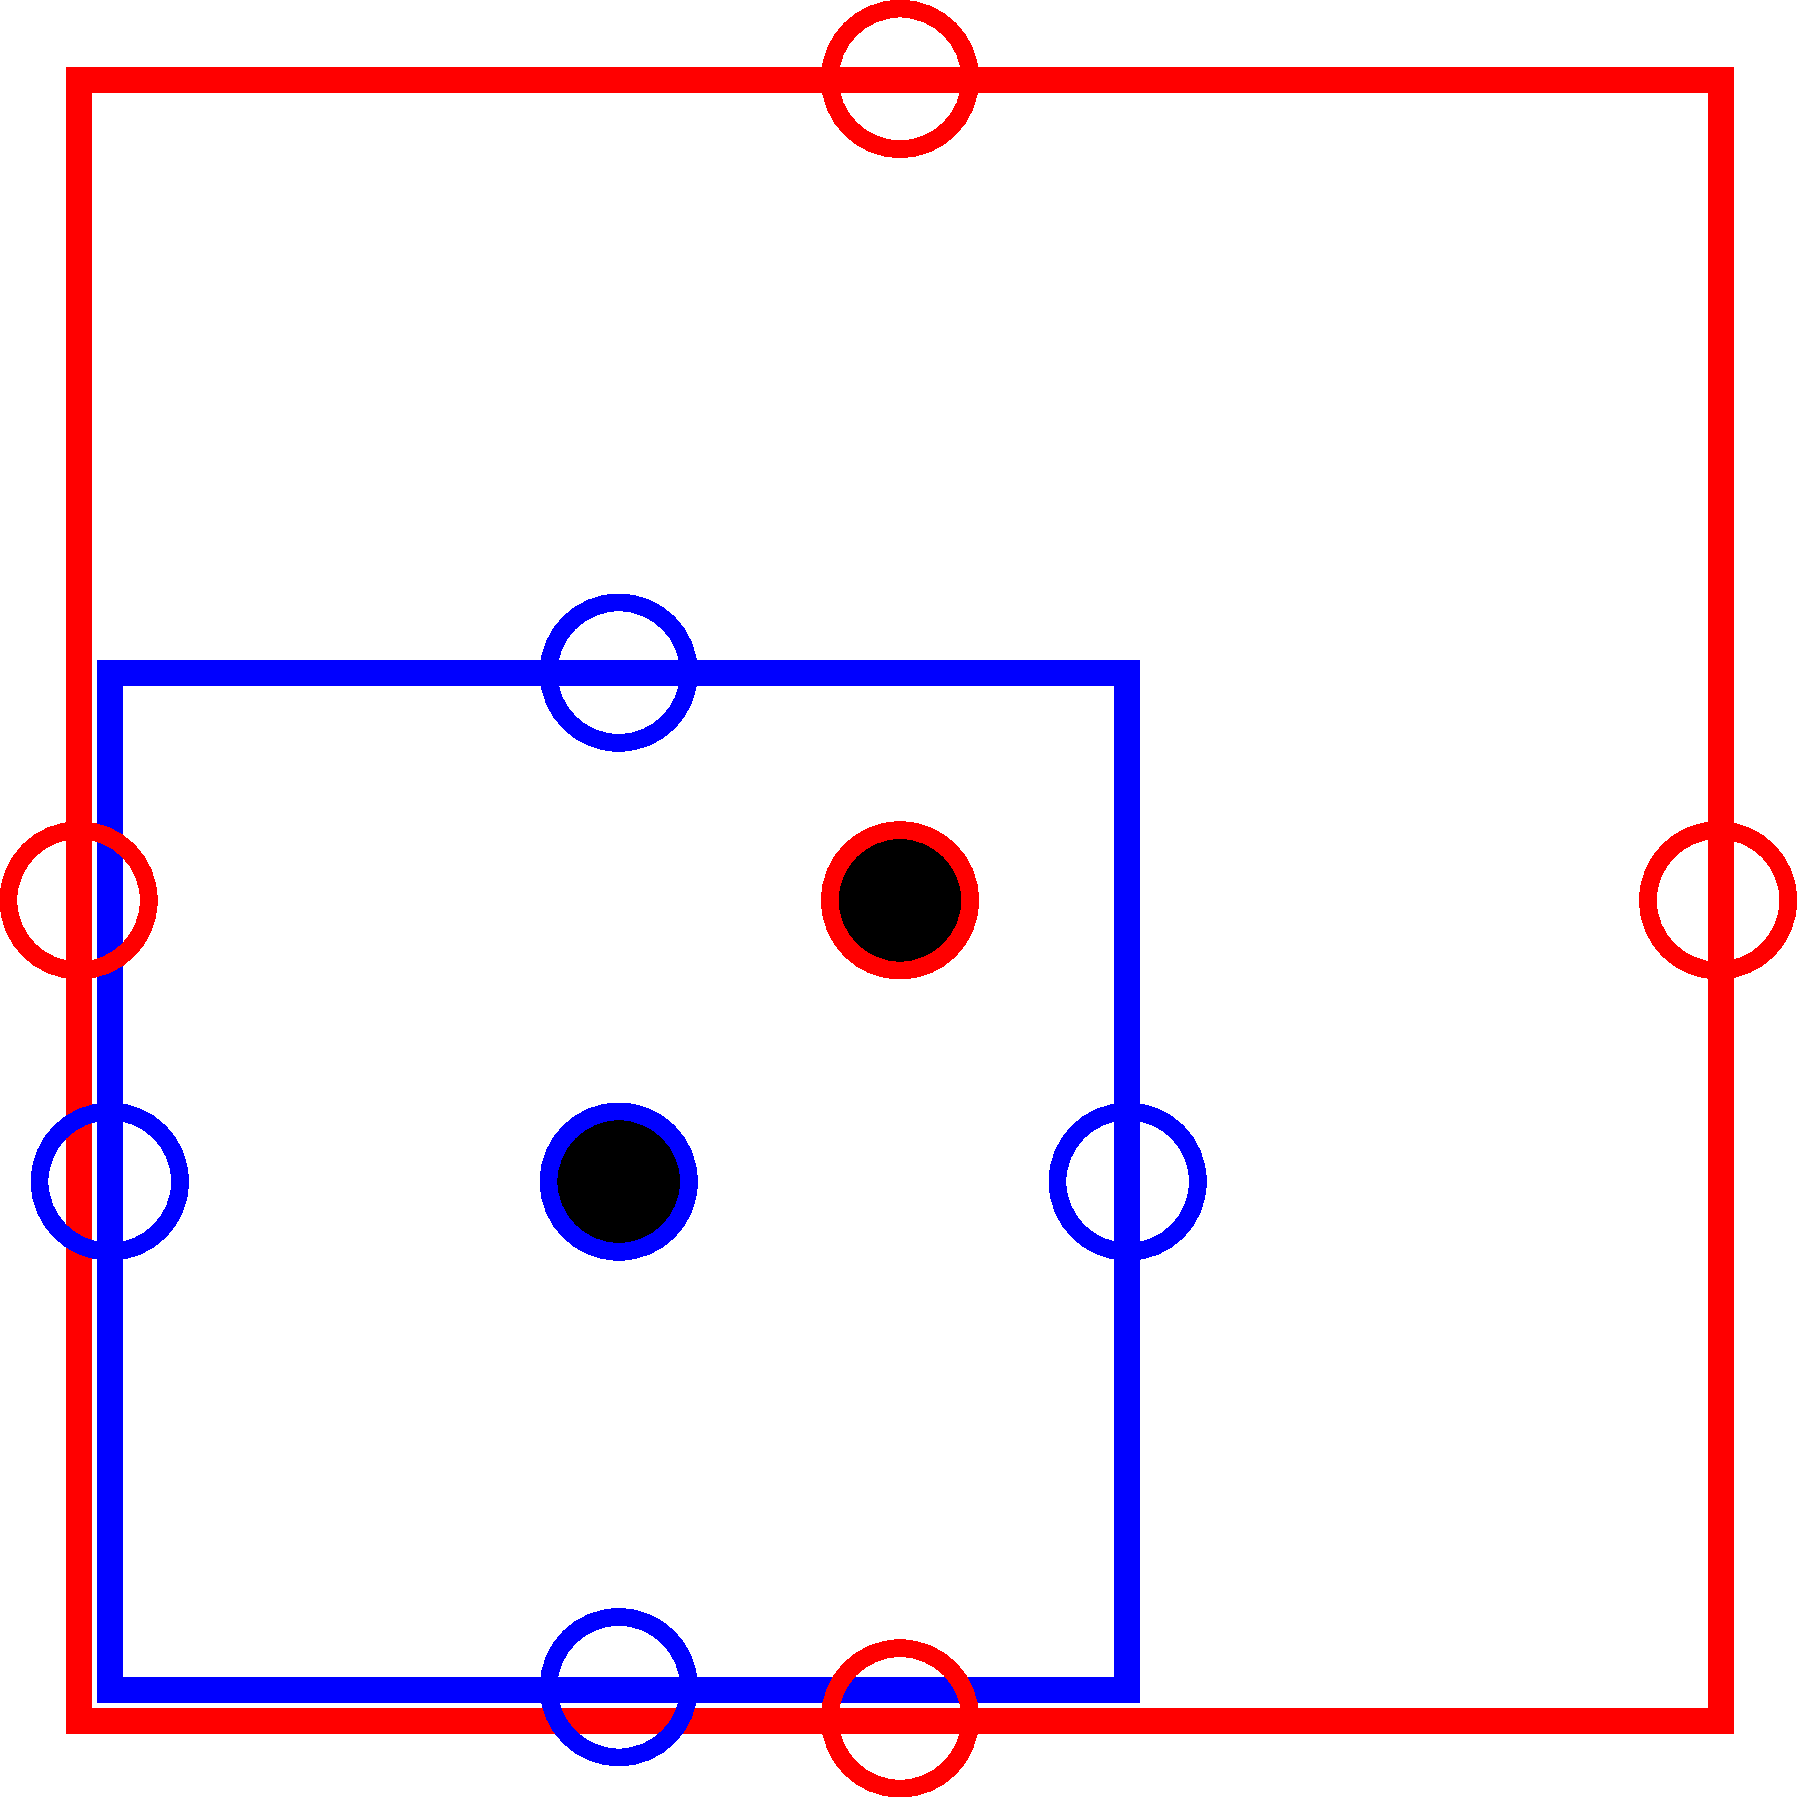
\includegraphics[width=0.6\textwidth]{drawings/audtestsetup}
    \caption{The setup for Room 1 and Room 2 (illustration of \Cref{fig:audtest}). Room 1 is marked as the inner (blue) square and is $5 \times 5$ meters. Room 2 is marked as the outer (red) square and is $8 \times 8$ meters. The rings shows the position of the beacons. The filled circles shows where the the phone is placed to obtain the position (only for the non-moving tests).}
    \label{fig:audtestsetup}
\end{figure}

\FloatBarrier
\subsection{Room 2}

\subsection{Room 3}

\subsection{Room 4}

\subsection{Conclusion}


We setup a [SIZE OF ROOM] room, with [NUMBER OF BEACONS]. 
The room is illustrated by \Cref{fig:precisiontest}. 
In \Cref{fig:precisiontest} you can also see small spots. 
These spots is the known locations where we are going to perform the precision tests. 
We randomly walk between these spots [NUMBER OF TIMES] and find the mean error rate.
\begin{figure}[!htb]
    \centering
    \todo[author=Thalley]{Insert figure}
    \caption{Illustration of room used for indoor location precision test}
    \label{fig:precisiontest}
\end{figure}

The mean error rate that we found is [RESULT]. 

\subsection{Precision of Indoor Location Conclusion}
From the results, we can conclude that... \todo[author=Thalley]{Write conclusion of precision test based on results}


\section{Overall System Correctness}\label{sec:systemcorrectness}
This test is designed to test the system as a whole. 
We want to test how many times the system:
\begin{enumerate}
    \item Sends the right action to the right device
    \item Sends the wrong action to the right device
    \item Sends the right action to the wrong device
    \item Sends the wrong action to the wrong device
\end{enumerate}
Thus this test is meant to total correctness of our system. 

We have the following setup, also illustrated in \Cref{fig:totalcorrectness}:
[SETUP: Which devices, where they are, where we stand, etc.]
\begin{figure}[!htb]
    \centering
    \todo[author=Thalley]{Insert figure}
    \caption{Illustration of our setup for the total correctness test}
    \label{fig:totalcorrectness}
\end{figure}

We send a total of [NUMBER OF GESTURES]. 
\Cref{table:correctnessresults} shows the results of this test.

\begin{table}
    \centering
    \begin{tabular}{l|cc}
                     & Right action & Wrong Action \\ \hline
        Right Device &      x       &     z        \\
        Wrong Device &      y       &     w        \\
    \end{tabular} 
    
    \todo[author=Thalley]{Insert results}
    \caption{Table showing the correctness of our system}
    \label{table:correctnessresults}
\end{table}

\subsection{Overall System Correctness Conclusion}
From the results, we can conclude that... \todo[author=Thalley]{Write conclusion of precision test based on results}

\section{Conclusion}
\begin{frame}{Conclusion}{Problem Statement}
  \begin{framed}
    How can wearables be utilized for home automation in a gesture driven solution?
  \end{framed}
  
  \begin{itemize}
    \item<2-> Developed a system that can control a smart home using a wearable
    \item<2-> Utilizes BLE beacons for indoor positioning
    \item<2-> Points at the correct devices \perc{4.29} of the time
    \item<2-> However, if we exclude the numbers from Room 3, we get
    \begin{itemize}
      \item<2-> An average position accuracy of \SI{2.1}{\meter}
      \item<2-> Corresponds to \perc{\sim12.5} correctness rate
    \end{itemize}
    \item<2-> We need a position accuracy of \SI{\sim 0.6}{\meter} to meet our requirement
  \end{itemize}
\end{frame}

%Thalley: Tænker lidt at slides med de spændende future works bliver for kedelige at se på
\begin{frame}{Future Work}
  \begin{enumerate}
    \item Use a wearable
    \item Investigate Alternatives for Indoor Positioning 
    \item Include Information About the User's Context
    \item Configuration of Locations
    \item Improve Detection of Pointing
    \item Continuous Recognition of Gestures
    \item 3-Dimensional Positions
    \item Support for more than binary gestures
  \end{enumerate}
\end{frame}


\end{document}

%%% Local Variables:
%%% mode: latex
%%% TeX-master: t
%%% End:
